Segundo Leonhardt Euler, o fator mais importante que determina a carga crítica nos elementos comprimidos é a \textbf{esbeltez}. Em função dela, conclui-se que, quanto mais esbelto for o elemento estrutural, menor será sua carga crítica.

A determinação do parâmetro \textbf{esbeltez} ($\lambda$) de um elemento estrutural é função do seu momento de inércia ($I$) de sua seção transversal, que é determinado em função de sua espessura. A propriedade da seção transversal que é usada na determinação da carga crítica é o \textbf{raio de giração da seção transversal} ($i$), que é relativo ao \textbf{momento de inércia}.
\begin{equation}i=\sqrt{\frac{I}{A}}\end{equation}

Onde $i$ é o raio de giração da seção geométrica da peça, sem considerar a presença da armadura; $I$ é o momento de inércia da seção transversal do pilar em relação ao eixo $x$ ou $y$; e $A$ é a área da seção transversal do pilar.

O momento de inércia indica a dificuldade de uma peça girar no eixo escolhido.

Para um pilar em pé em relação à visão em planta:

\begin{figure}[H]
	\begin{center}
	\caption{Exemplo de seção transversal (retangular) para cálculo do momento de inércia.}
    	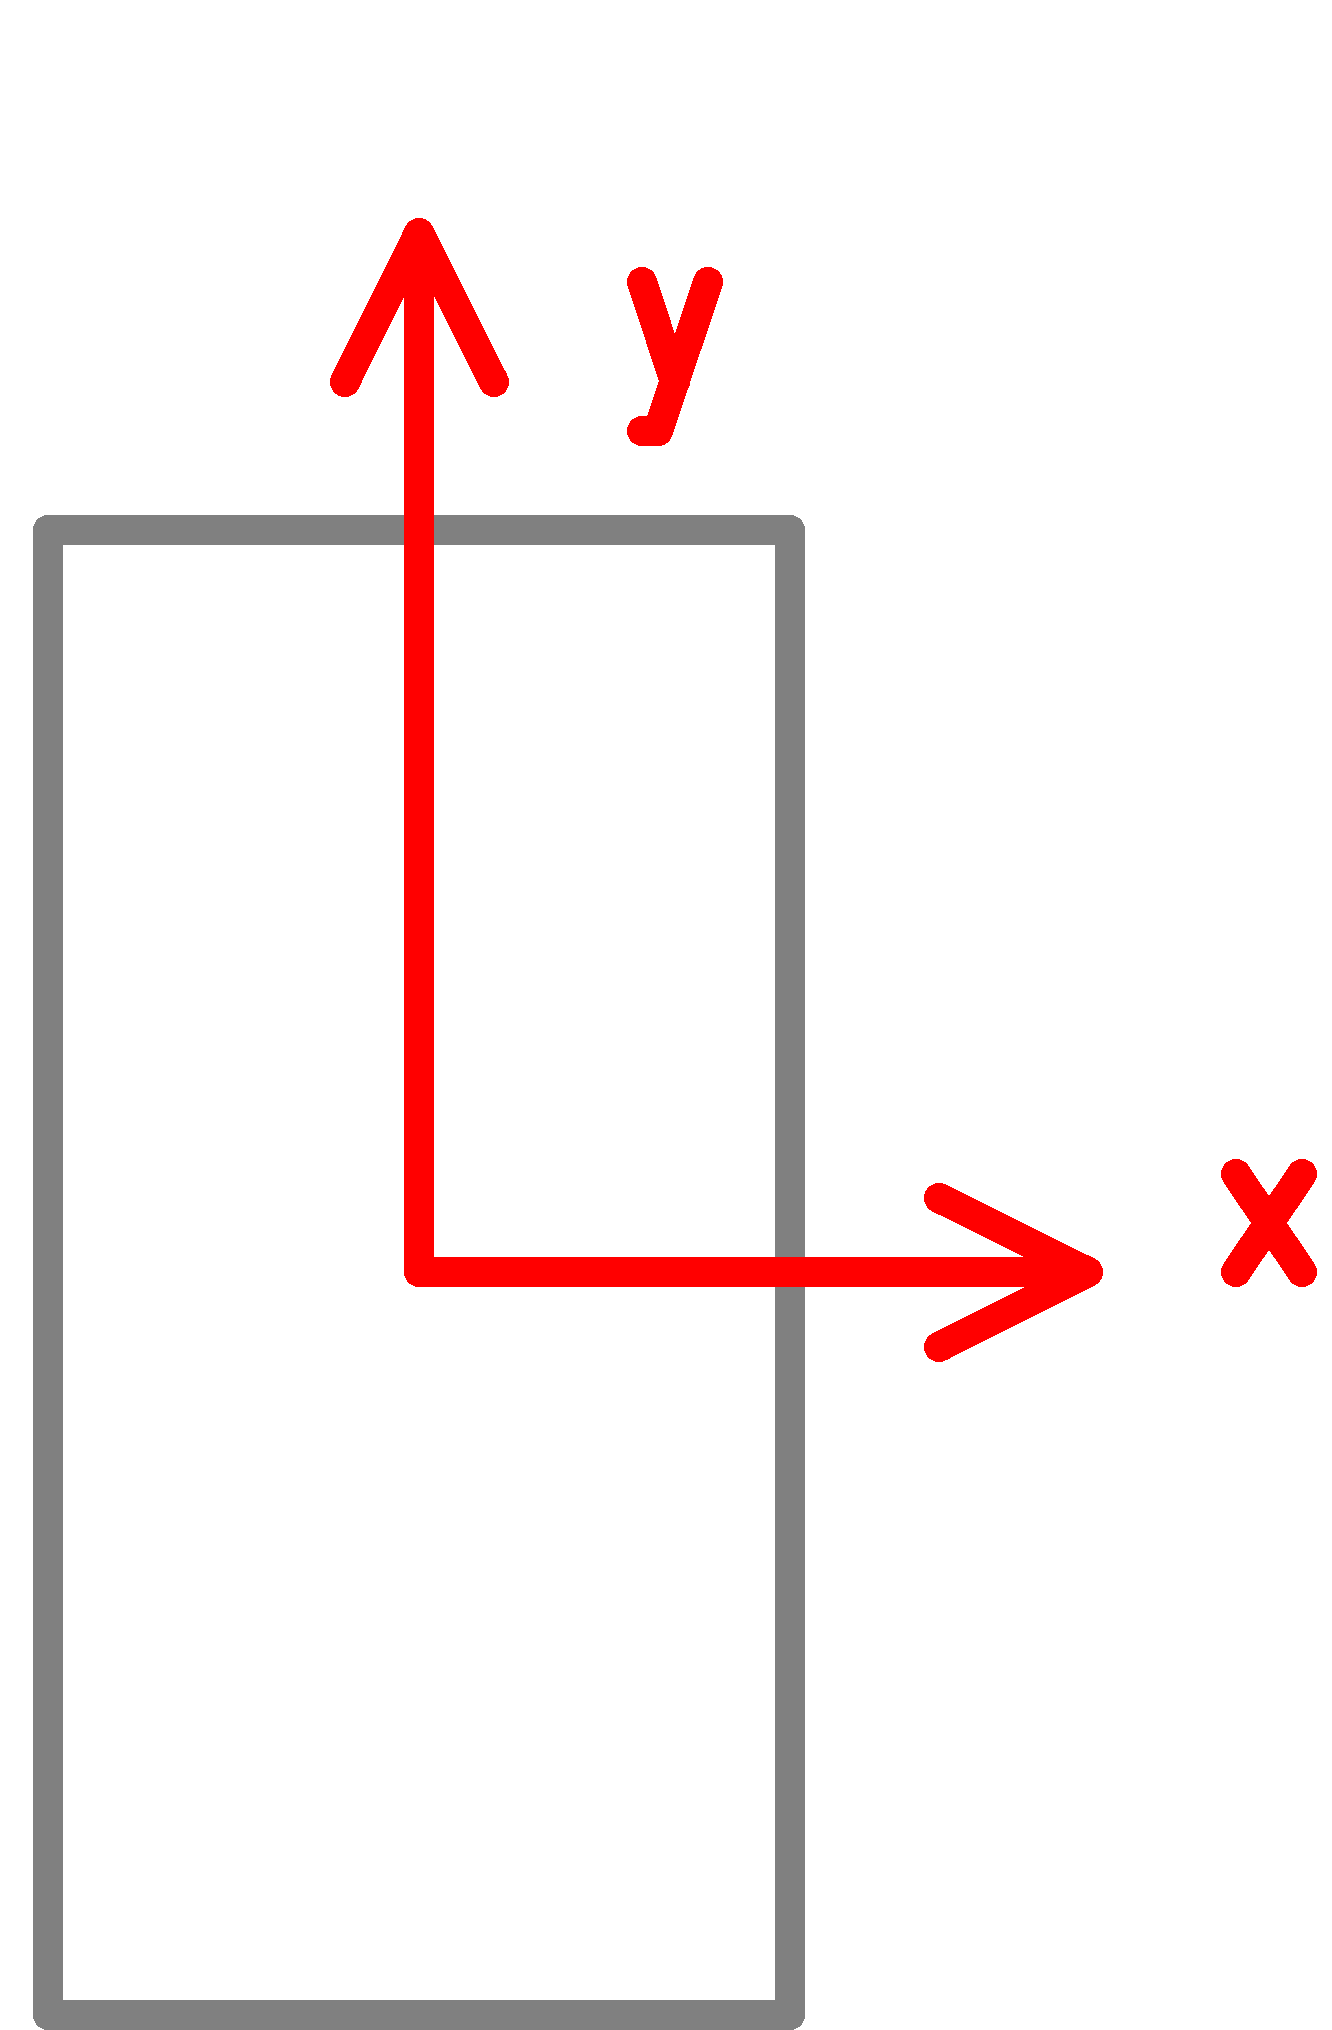
\includegraphics[width=0.1\textwidth]{Indice-de-esbeltez/Imagens/Secao-transversal-pilar.png}
	\end{center}
\end{figure}

Na direção $x$ (a base será sempre a face onde o eixo está olhando). Por exemplo, um pilar $P1$ (20x70):
$$I_x=\frac{b\cdot h^3}{12}=\frac{70\cdot{20}^3}{12}\approx46666,6667\;{cm}^4$$

E na direção $y$:
$$I_y=\frac{b\cdot h^3}{12}=\frac{20\cdot{70}^3}{12}\approx571666,6667\;{cm}^4$$

Ou seja, é muito mais difícil rotacionar no eixo $y$.